\subsection{Stoichiometry}
Source: \href{https://www.youtube.com/watch?v=UL1jmJaUkaQ&list=PL8dPuuaLjXtPHzzYuWy6fYEaX9mQQ8oGr&index=7}{Stoichiometry - Chemistry for Massive Creatures: Crash Course Chemistry \#6}
\\\\
Stoichiometry is the relationship between the quantities of reactants and products before, during, and following chemical reactions.

\begin{description}
    \item[amu] $1.66 \cdot 10^{-27}kg =$ 1/12 the mass of an atom of $^{12}C$
    \item[mol] $6.022 \cdot 10^{23}$ (Avogadro's number)
    \item[Relative atomic mass] ram (deprecated atomic weight) is the ratio to the atomic mass unit (amu)
    \item[Molar mass] $\text{mol} \cdot \text{Relative atomic mass} =$ (Weight of one mol of the element)
    \item[Molarity] $M = \dfrac{\text{solute in moles}}{\text{solution\space in\space liters}}$
    \item[Molality]  $m = \dfrac{\text{solute in moles}}{\text{kg of solution}}$
    \item[Equation balancing] atom on lhs = atoms on rhs\\
        %$C_{12}H_{22}O_{11} + 12 O_{2} = 12 CO_{2} + 11 H_{2}O$\\
        $\sucrose + 12\oxygen = 12\carbonDioxide + 11\water$\\
        It means that to burn 5g of sucrose you need 5.6g of oxygen $\approx$ 35 breaths
\end{description}
%
Weight of one mol of $\sucrose = \text{C} + \text{H} + \text{O}$\\
$\text{C} = 12 \text{mol} \cdot 12.01\text{g/mol} = 144.12\text{g}$\\
$\text{H} = 22 \text{mol} \cdot 1.008\text{g/mol} = 22.176\text{g}$\\
$\text{O} = 11 \text{mol} \cdot 16.00\text{g/mol} = 171\text{g}$\\
One mol of sucrose = 342.296g

\subsubsection{Exothermic \& Endothermic}
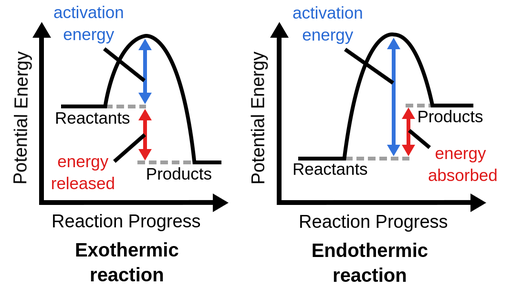
\includegraphics[width=30em]{./includes/chemistry/imgs/exo_endo.png}